\newpage
\subsubsection{Acidity} \label{sensors:acidity}

As mentioned in the Design Report, the DFRobot SEN0169 V2 Pro \cite{SEN0169V2} was chosen for measuring the acidity. The manufacturer claims the sensor has a resolution of 0.1pH across the whole range from 0 to 14pH.

\begin{figure}[h]
  \centering
  \begin{minipage}[b]{0.4\textwidth}
    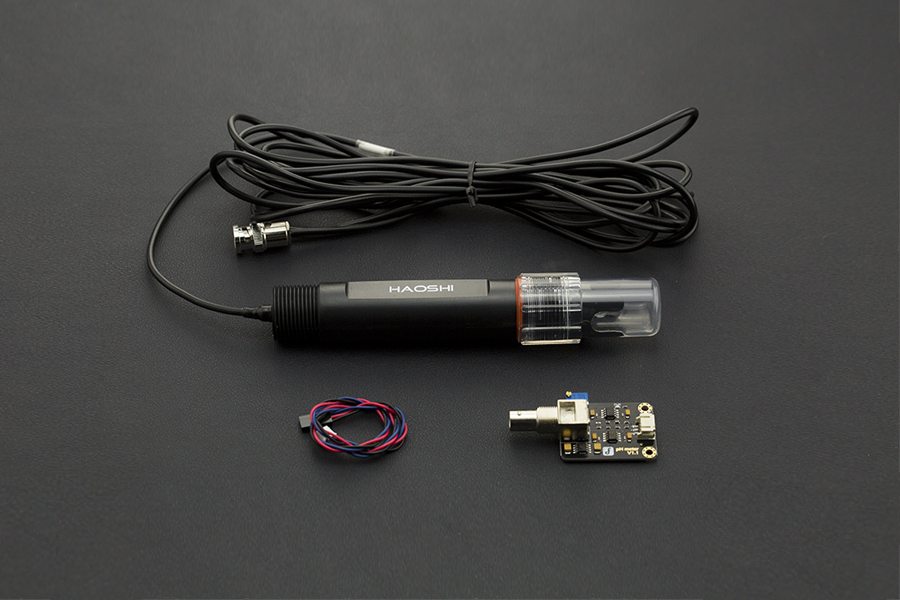
\includegraphics[width=\textwidth]{080_testing/sensors/12_gravityv2pro.jpg}
    \caption{SEN0169 V2 Pro \cite{SEN0169V2}}
  \end{minipage}
  \hfill
  \begin{minipage}[b]{0.3\textwidth}
    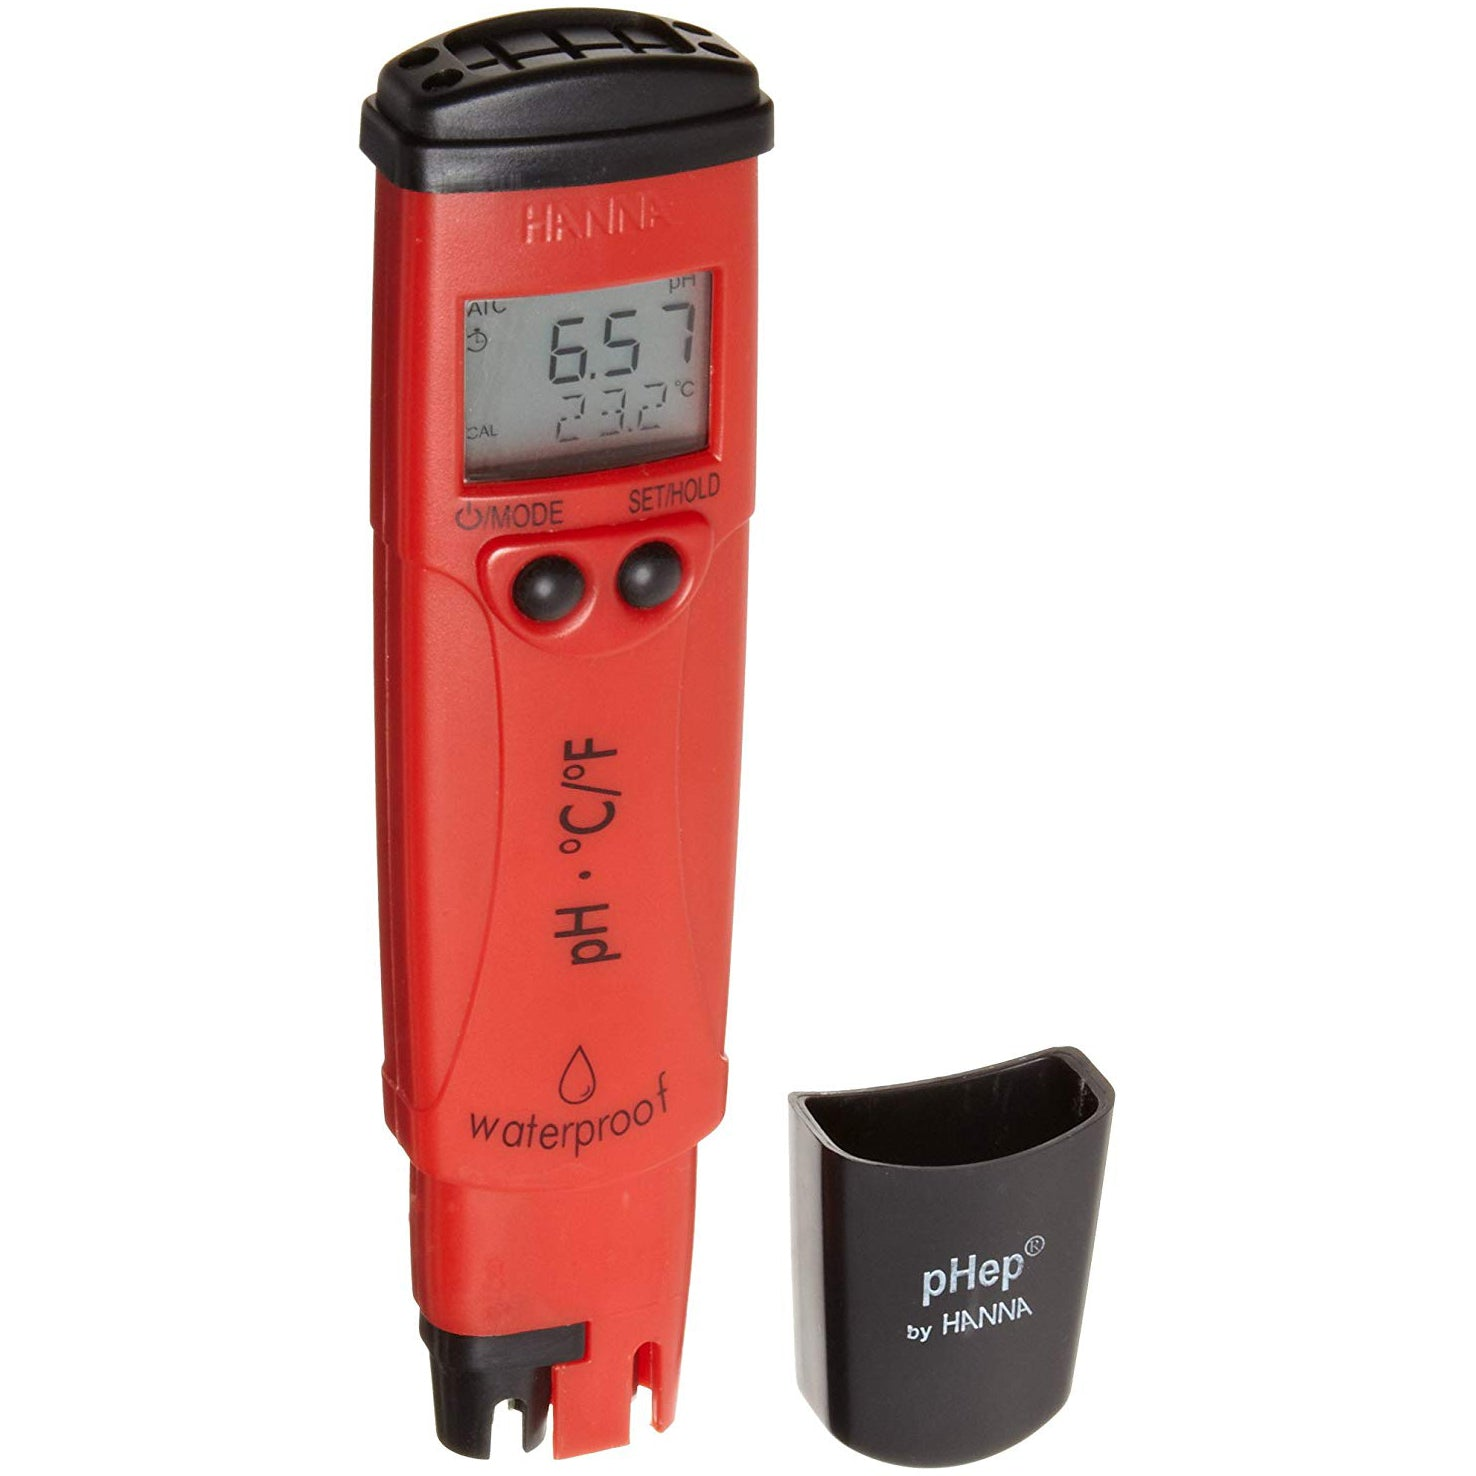
\includegraphics[width=\textwidth]{080_testing/sensors/11_hanna.jpg}
    \caption{Hanna pHep \cite{hanna}}
  \end{minipage}
\end{figure}

The chosen sensor was compared against the Hanna pHep, that also has a resolution of 0.1pH. \cite{hanna} Two solutions with different pH were tested on both sensors. Before each sample was taken, both sensors were cleaned with distilled water. A sample is taken a minute after submersion, as the response time of both acidity sensors are within 1 minute.

\newpage
\paragraph{First solution}
The first solution is marked in pink.

\begin{figure}[h]
  \centering
  \begin{minipage}[b]{0.2\textwidth}
    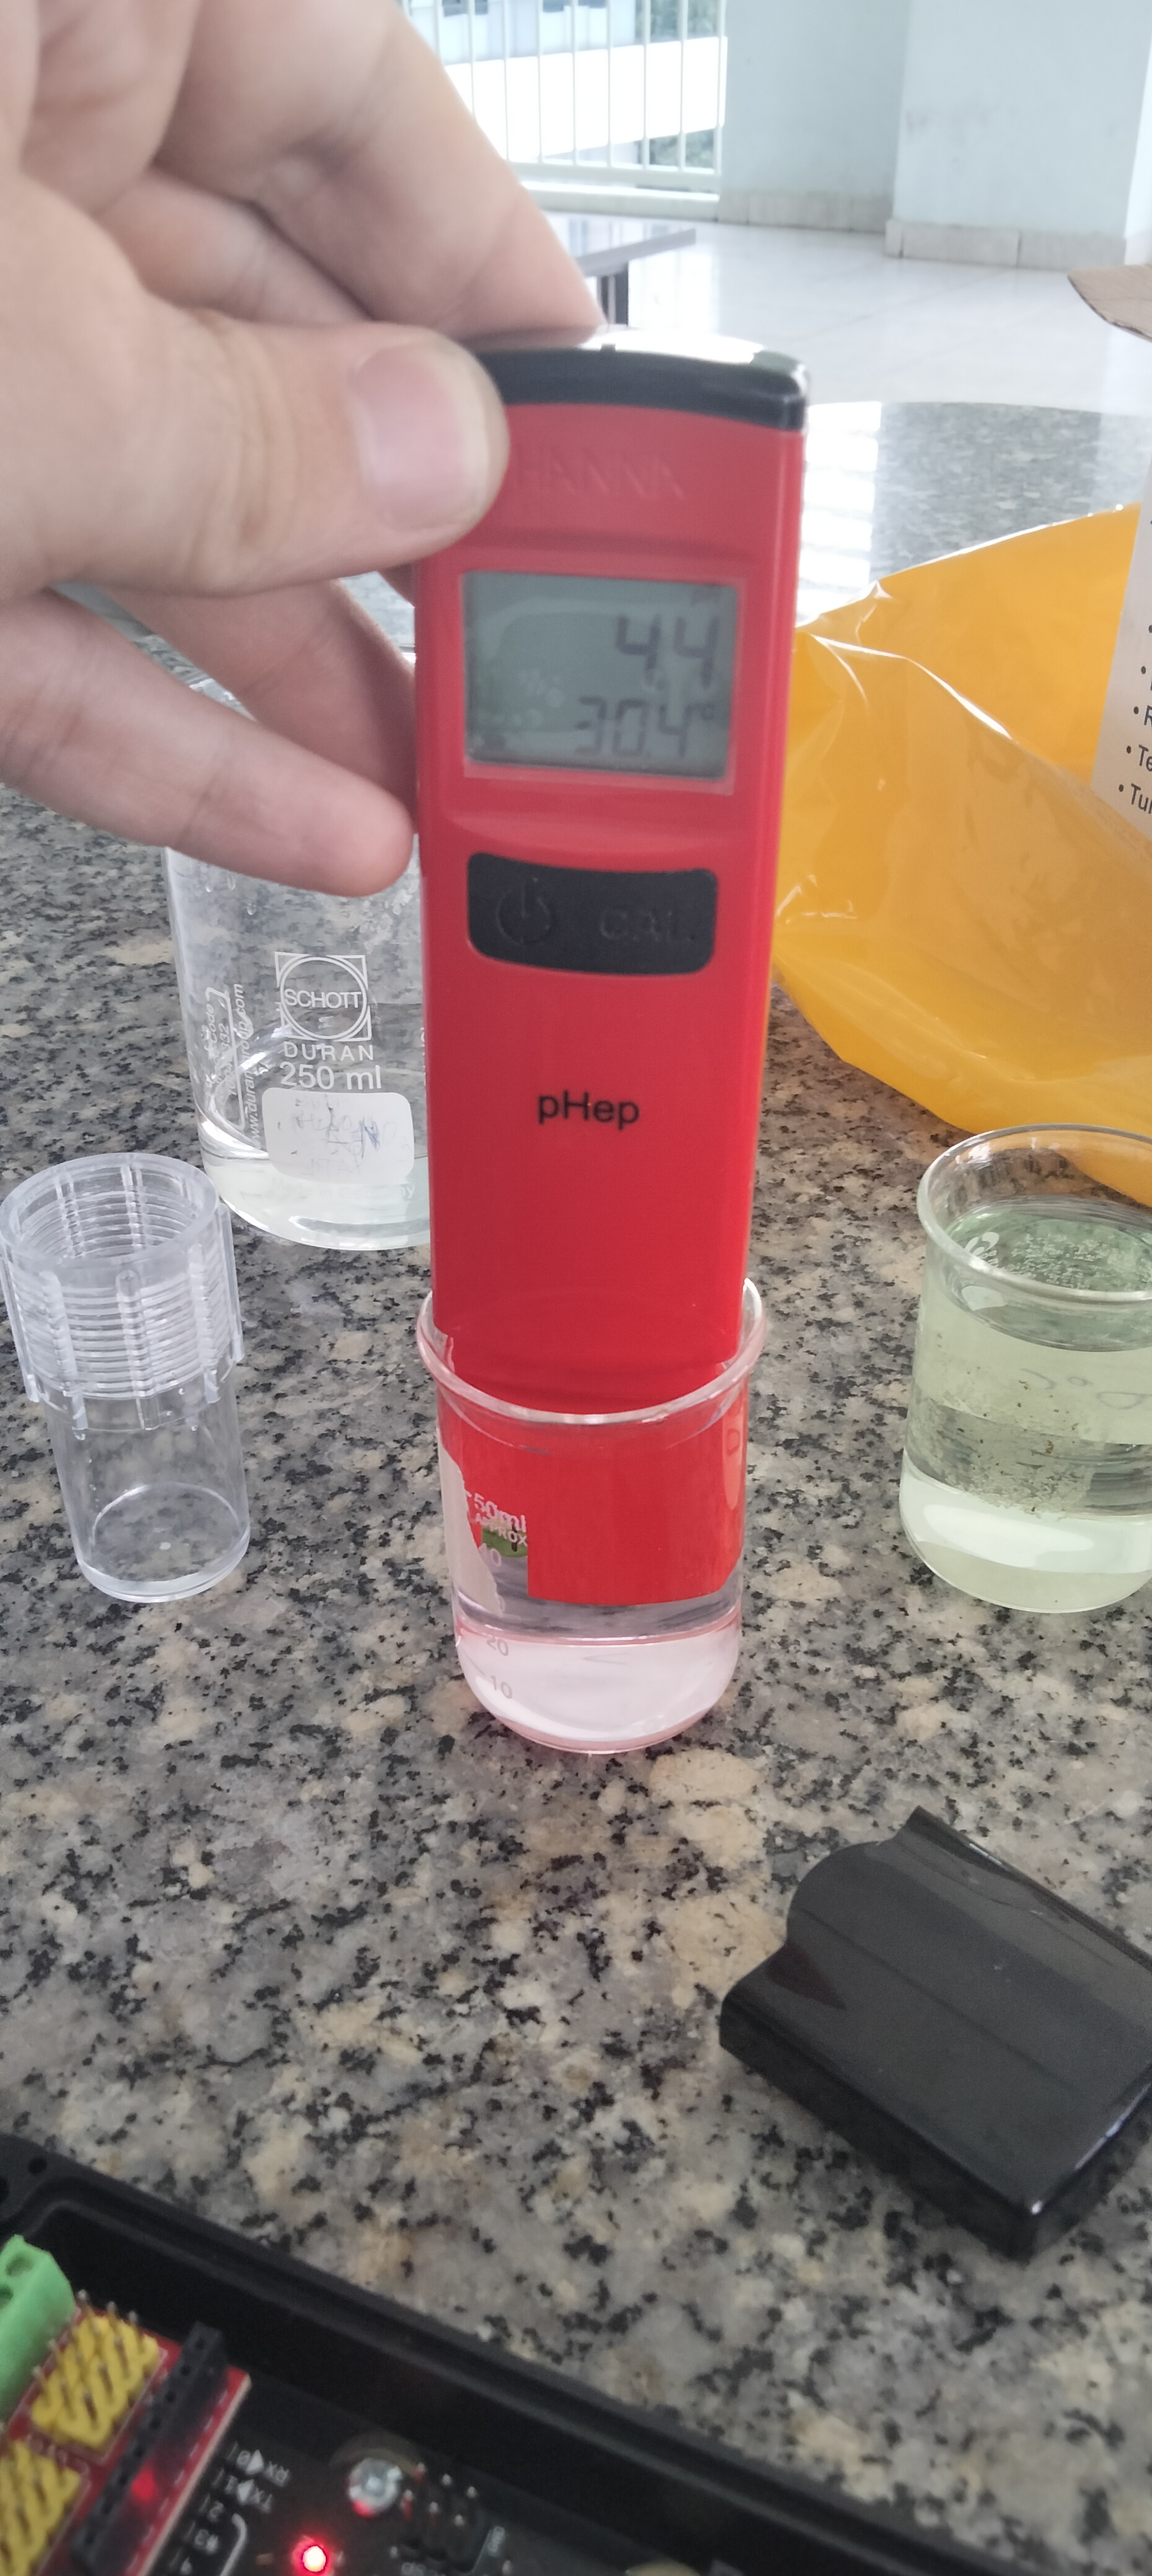
\includegraphics[width=\textwidth]{080_testing/sensors/14_ph4_hanna.jpg}
    \caption{Hanna sensor measuring 4.4 [own picture]}
  \end{minipage}
  \hfill
  \begin{minipage}[b]{0.7\textwidth}
    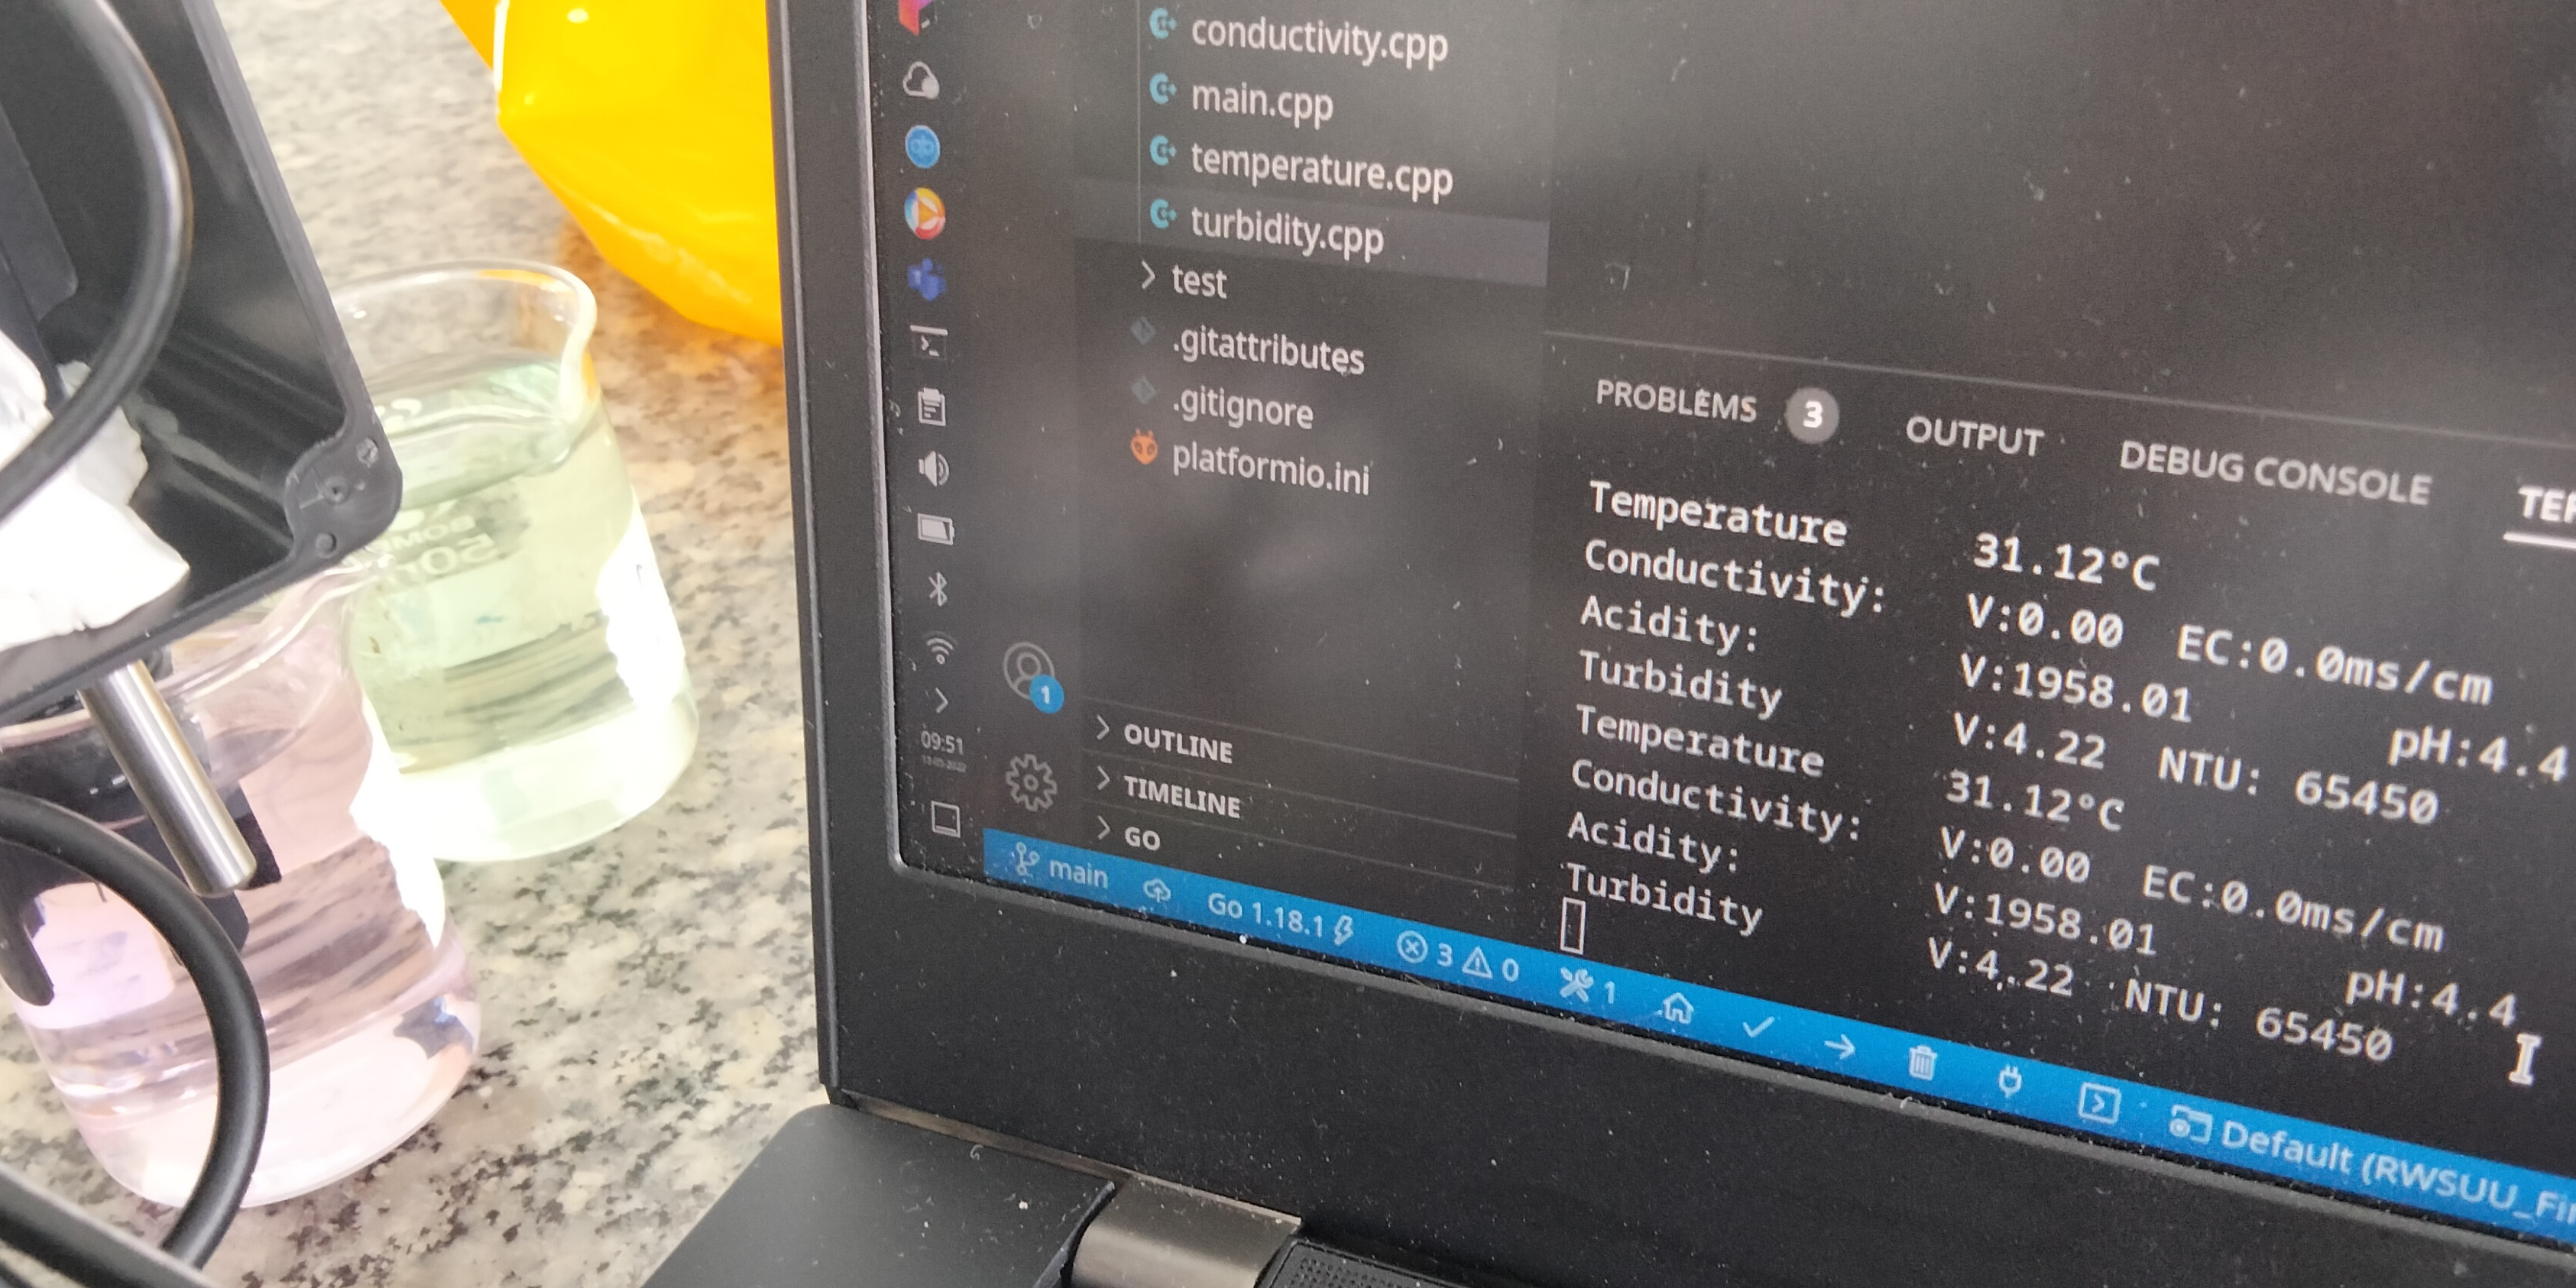
\includegraphics[width=\textwidth]{080_testing/sensors/13_ph4_dfrobot.jpg}
    \caption{DFRobot sensor measuring 4.4 [own picture]}
  \end{minipage}
\end{figure}

\begin{figure}[h!]
\caption{Comparison between Hanna and DFRobot on pH 4.4}
\begin{tikzpicture}
\begin{axis}[
axis lines=middle,
ymin=0,
x label style={at={(current axis.right of origin)},anchor=north, below=10mm},
legend style={at={(0.7,0.7)},anchor=east},
ymin=4, ymax=5,
    xlabel=Samples,
  ylabel=pH,
   enlargelimits = true,
  xticklabels from table={ph4.dat}{Sample},xtick=data]
\addplot[orange,thick,mark=square*] table [y=Hanna,x=X]{ph4.dat};
\addlegendentry{Hanna}
\addplot[green,thick,mark=square*] table [y= DFRobot,x=X]{ph4.dat};
\addlegendentry{DFRobot}]
\end{axis}
\end{tikzpicture}
\end{figure}

As seen in the graph above, both sensors repeatedly measured a pH of 4.4. The DFRobot sensor read 4.3 on the first sample, this falls within the indicated margin of error.

\newpage
\paragraph{Second solution}
The second solution is marked in light yellow. The Hanna pHep repeatedly measured a pH of 7.2, while the DFRobot sensor repeatedly measured a pH of 7.3

\begin{figure}[h]
  \centering
  \begin{minipage}[b]{0.2\textwidth}
    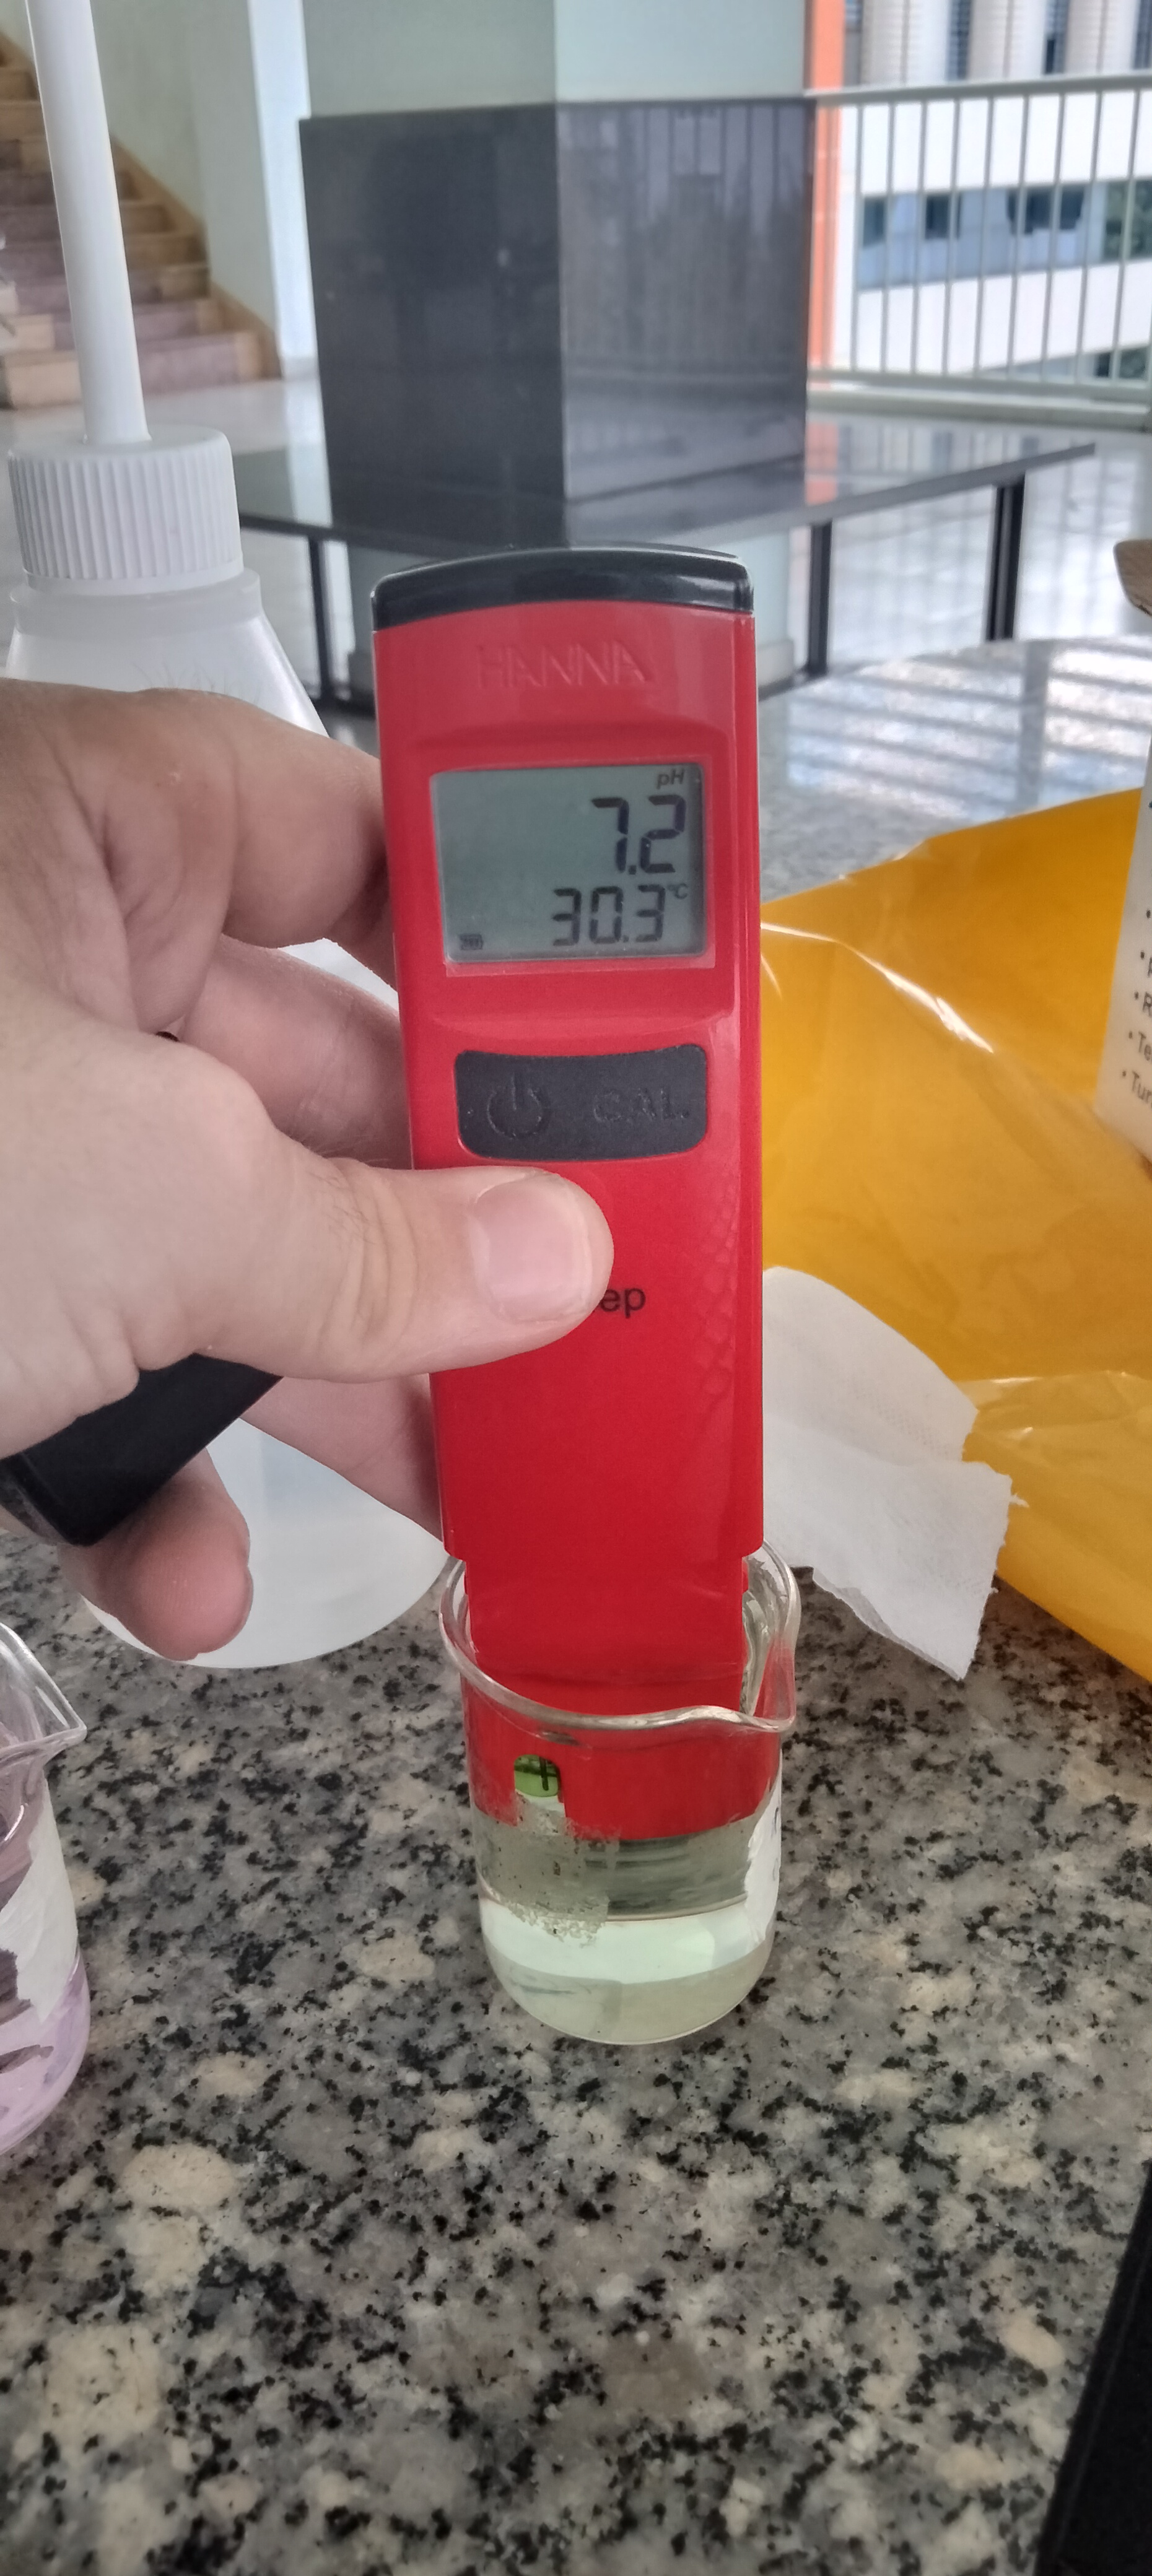
\includegraphics[width=\textwidth]{080_testing/sensors/16_ph7_hanna.jpg}
    \caption{Hanna sensor measuring 7.2 [own picture]}
  \end{minipage}
  \hfill
  \begin{minipage}[b]{0.7\textwidth}
    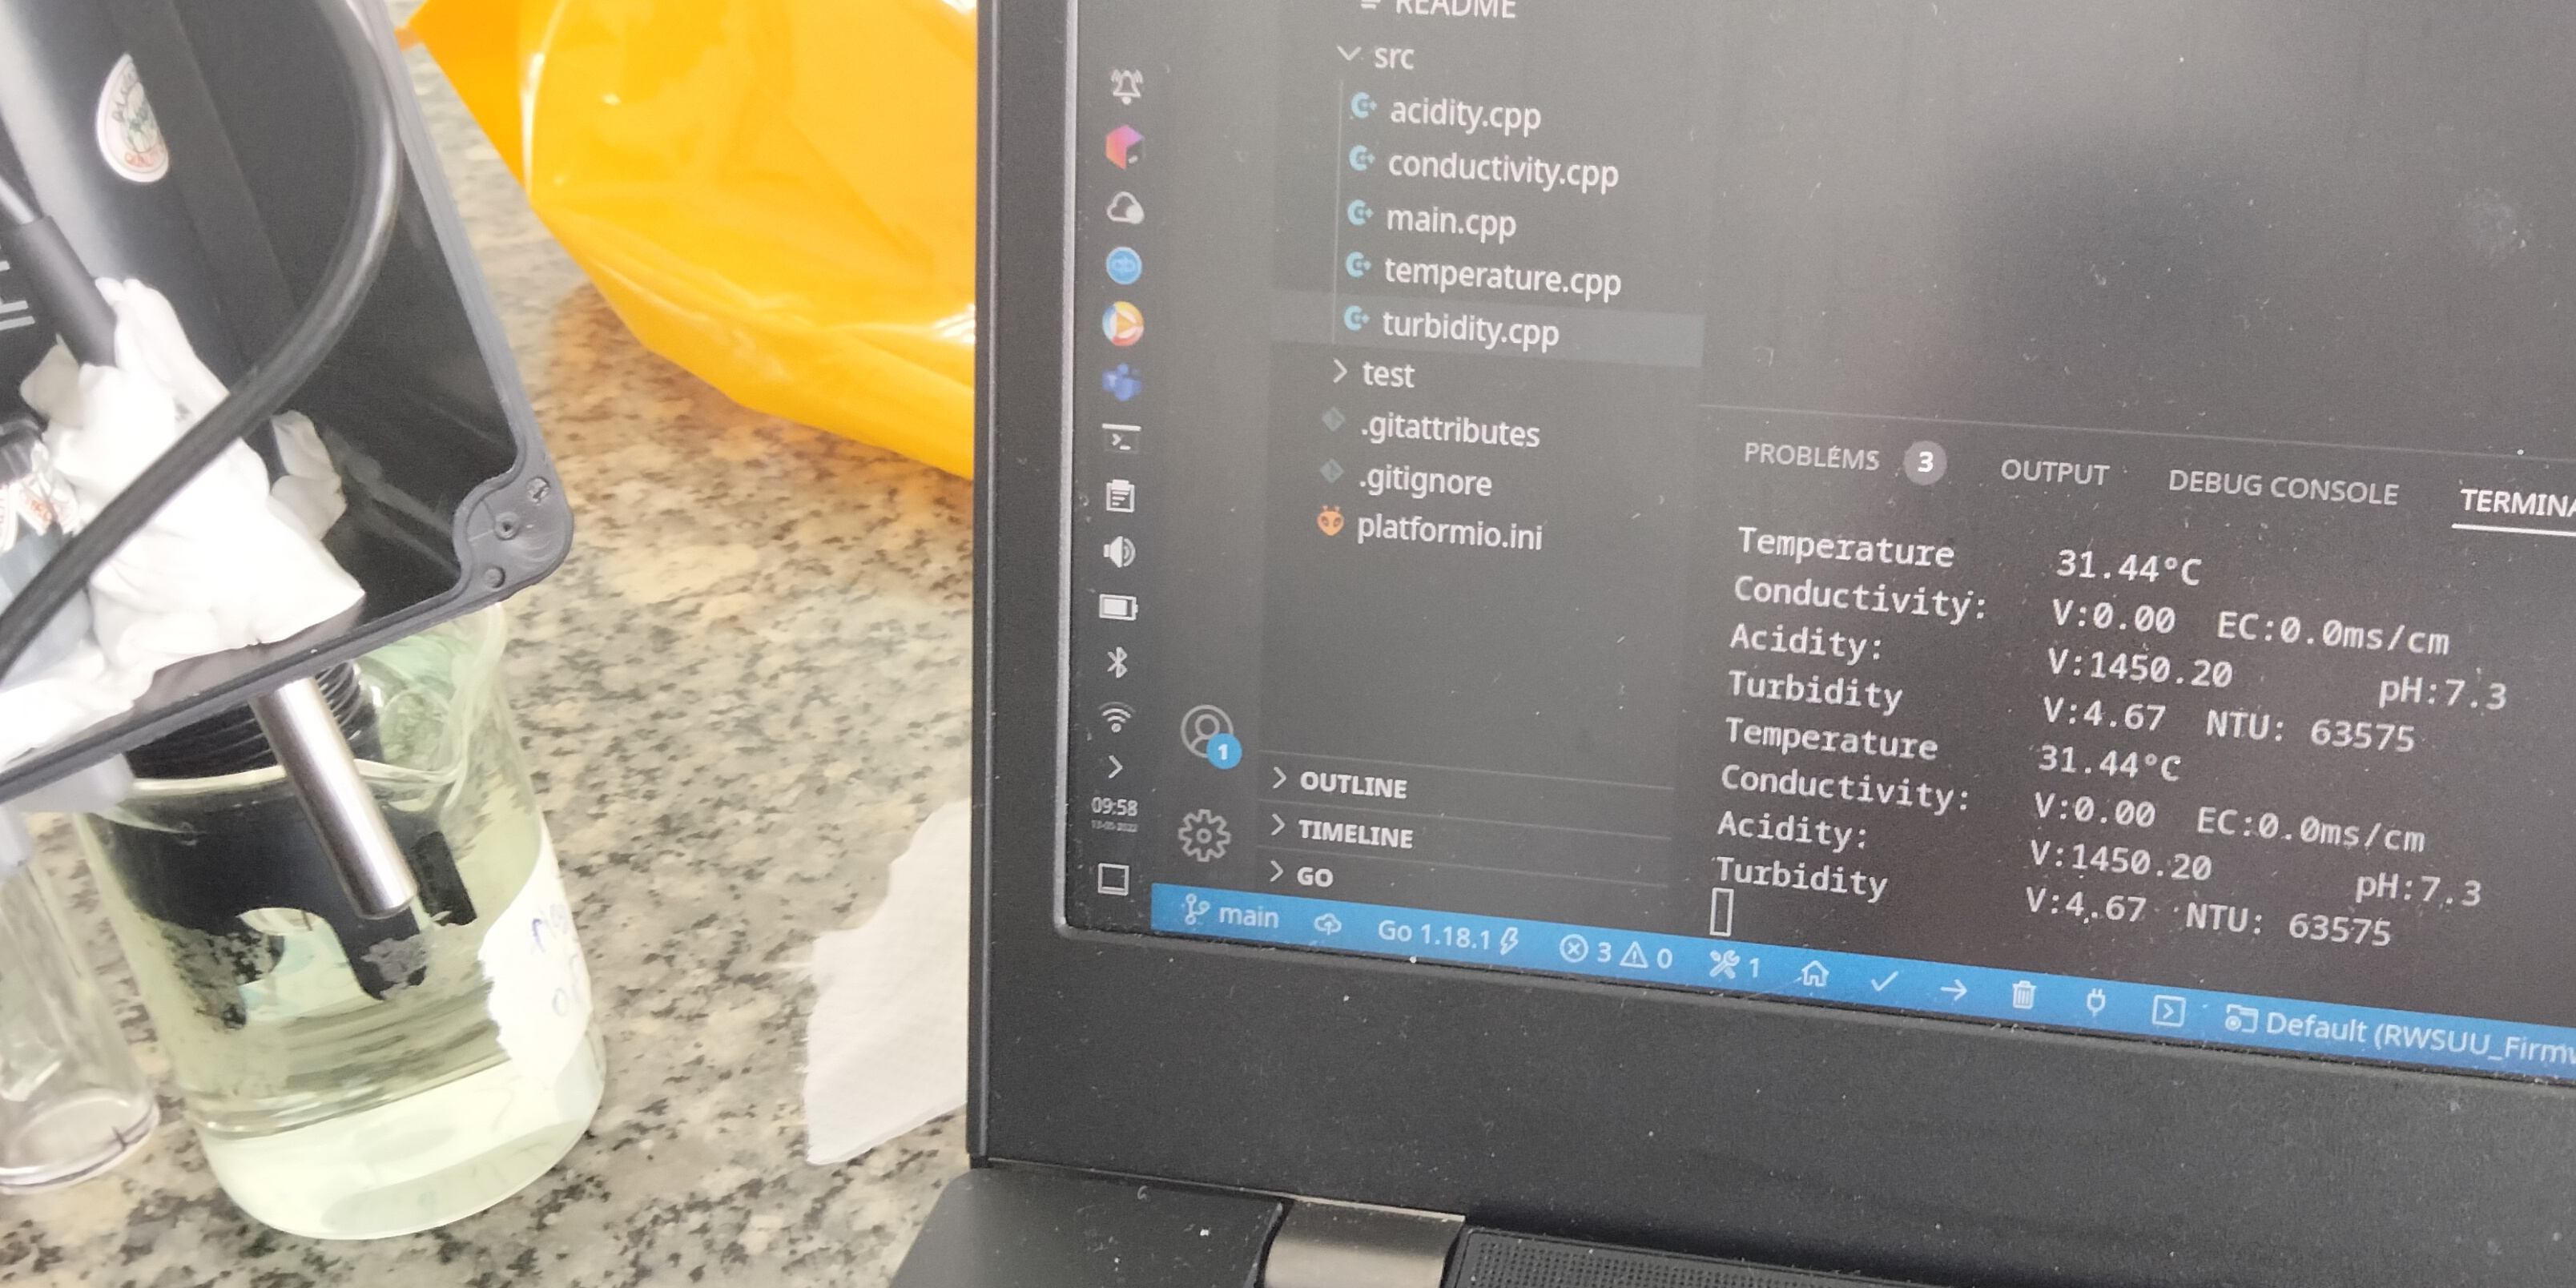
\includegraphics[width=\textwidth]{080_testing/sensors/15_ph7_dfrobot.jpg}
    \caption{DFRobot sensor measuring 7.3 [own picture]}
  \end{minipage}
\end{figure}

\begin{figure}[h!]
\caption{Comparison between Hanna and DFRobot on pH 7.2}
\begin{tikzpicture}
\begin{axis}[
axis lines=middle,
ymin=0,
x label style={at={(current axis.right of origin)},anchor=north, below=10mm},
legend style={at={(0.7,0.7)},anchor=east},
ymin=7, ymax=8,
    xlabel=Samples,
  ylabel=pH,
   enlargelimits = true,
  xticklabels from table={ph4.dat}{Sample},xtick=data]
\addplot[orange,thick,mark=square*] table [y=Hanna,x=X]{ph7.dat};
\addlegendentry{Hanna}
\addplot[green,thick,mark=square*] table [y= DFRobot,x=X]{ph7.dat};
\addlegendentry{DFRobot}]
\end{axis}
\end{tikzpicture}
\end{figure}

As seen in the graph above, the Hanna sensor continously reads 7.2, while the DFRobot sensor continously reads 7.3. The exception is the fourth sample, when the Hanna sensor also read 7.2. This falls into the indicated margin of error.